%%==================================================
%% chapter02.tex for SJTU Bachelor Thesis
%% version: 0.5.2
%% Encoding: UTF-8
%%==================================================

\chapter{Basic Concepts and Backgrounds}
\label{chap:Basic Concepts and Backgrounds}

\section{Data Center Network}
\label{sec:Data Center Network}
Data Center Network is a certain kind of network that requires the collaboration in a global scale. Currently, the traffic inside a data center has the feature of centralized data exchanging \cite{dcnarch}, and the east-to-west traffic is increasing. Thus a data center is now required for a larger scale, high scalability, high robustness and effective network protocols. In this situation, the traditional 3-tier architecture is confronting many challenges. And now network flattening, network virtualization and a programmable structure is becoming the new trend of a DCN.

Among all the features required for current DCN, virtualization is what we used widely in data centers. It permits a single physical machine to hold several virtual machines, which are totally unrelated to each other. When one of these physical machines are processing too much work, its virtual machines will be dynamically moved to other physical machines that are not overloaded. This process will improve the performance of the whole network, by decreasing hot nodes. Meanwhile, as data centers becoming larger and larger, the scalability of DCN is also becoming more important. 

For a DCN, there are two problems to be considered. First, if we use a centralized server to allocate resources, the whole network will be down if that server breaks down. Second, Internet is a network to be used by a lot of users, all those users should have their own space. Thus, the data centers are currently designed in a distributed structure. Then in order to make better control of the network, SDN is born. In a network that has thousands of hosts, if we want to make the system balanced, we have to make a lot of migrations dynamically according to the traffic. If we allocate appropriate forwarding rules for each node in this migration process, the performance can be improved. In this way, we need a monitoring component to design such schemes according to different traffic.

Since traffic in DCN can be considered as migration of virtual machines, we have to deal with this problem quite frequently. To make the system balanced, we need a monitoring component, which can be regarded as a controller in SDN. And for each flow, it represents the communication between a pair of VM, which will go through some switches. Thus, in a DCN, controllers have to manage the flows among all switches, and that is the problem we want to discuss in this paper. To make it more practical and easier to understand, we deploy the OpenFlow framework in a data center network and design schemes accordingly.

\section{Concepts of SDN and OpenFlow}
\label{sec:Concepts of SDN and OpenFlow}

\subsection{The Element of SDN}
\label{sec:The Element of SDN}
SDN is a new kind of network model. In this model, the control part is separated from the hardware part that is responsible for forwarding data packets. This migration of the control plane leads to a logically centralized controller, which contributes to a more flexible and programmable framework. To deploy a Software Defined Network, several elements are necessary: SDN switches (e.g. OpenFlow switches), SDN controllers, the interface of the controller that is used for communicating with forwarding devices, the generally southbound interface (OpenFlow), and the Internet application interface (northbound interface). In SDN, since the controlling logic and the algorithms are migrated to the controller, switches are usually presented as basic forwarding hardware that can be visited via public interfaces.

The OpenFlow switches are divided into two types: pure OpenFlow switches (that only support OpenFlow operations) and hybrid OpenFlow switches  (that enables OpenFlow operations as well as other operations) \cite{openbook}. The pure OpenFlow switches do not have the character of on-board control that is supported by traditional switches, and is totally dependent on the controller to make forwarding decisions. The hybrid OpenFlow switches have strong functions. Apart from supporting OpenFlow operations, it also enables traditional operations and protocols. Most of the current commercial switches are hybrid switches.

Inside the OpenFlow switches there is a flow table. The flow table is responsible for data packet lookup and forwarding. Usually the flow table is empty the first time we launch SDN, and will save used routes as packets are passing by flooding in the beginning, if the controller is an layer two switch. Of course, the supervisor of the network can also input the routes in the flow table before the network starts, such that unncessary flooding can be avoided. In a flow table, there is a set of flow entries. The flow entries mainly consists of three parts: match fields, counters and instruction sets, as shown in Figure \ref{flowtable}. The match fields contains the information of the data packets, such as inport number, VLAN ID and metadata, which is used for matching inout packets. And the counter is used to collect the statistics of certain flows, such as the lasting time of the flow, the number of flows and the size of flows. The instruction sets are used for deciding how to manipulate the packets that match the conditions. The flow entries may exist for a certain amount of time that can be set in the beginning, and will be deleted after this time, in order to make spaces for new flow entries.

\begin{figure}[htbp]
  \centering
  % Requires \usepackage{graphicx}
  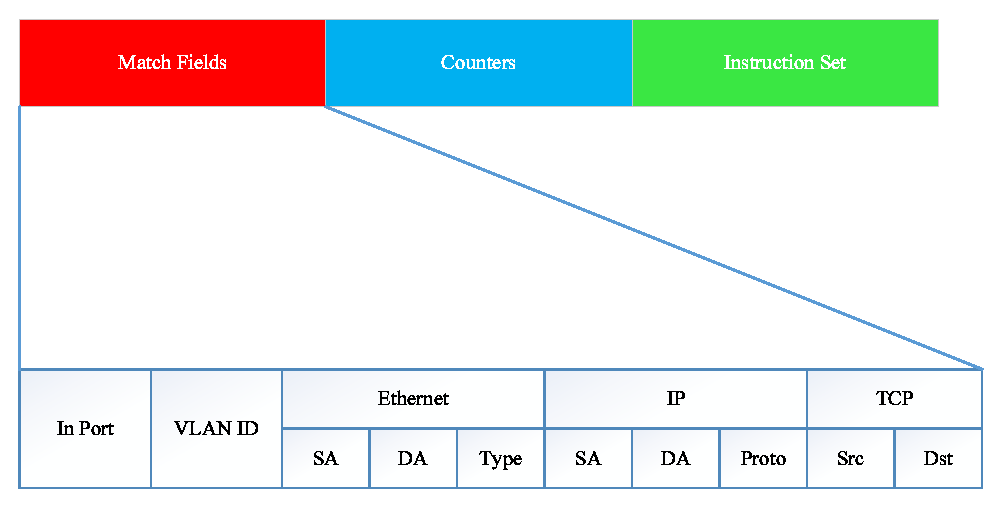
\includegraphics[scale=0.75]{chap2/flowtable.eps}
  \caption{The flow table of OpenFlow1.0}\label{flowtable}
\end{figure}

Everytime a packet reaches an OpenFlow switch, the header fields will be extracted, and compare will the matching field of the flow entries. The comparision starts from the first entry and continues in sequence. When a matching entry is found, the packet will be processed according to the corresponding schemes in that entry. Meanwhile, the value of counters will be modified when there is a match. If no matching entries are found, the switch will take actions refering to the table-missing records in the flow table. Each flow table must have a table miss record, in order to deal with situations where no match is found. In this record, a set of instructions will be defined, such as discarding the packet, flooding the packet, or forwarding the packet to the controller. The process is shown in Figure \ref{switchact}.

\begin{figure}[htbp]
  \centering
  % Requires \usepackage{graphicx}
  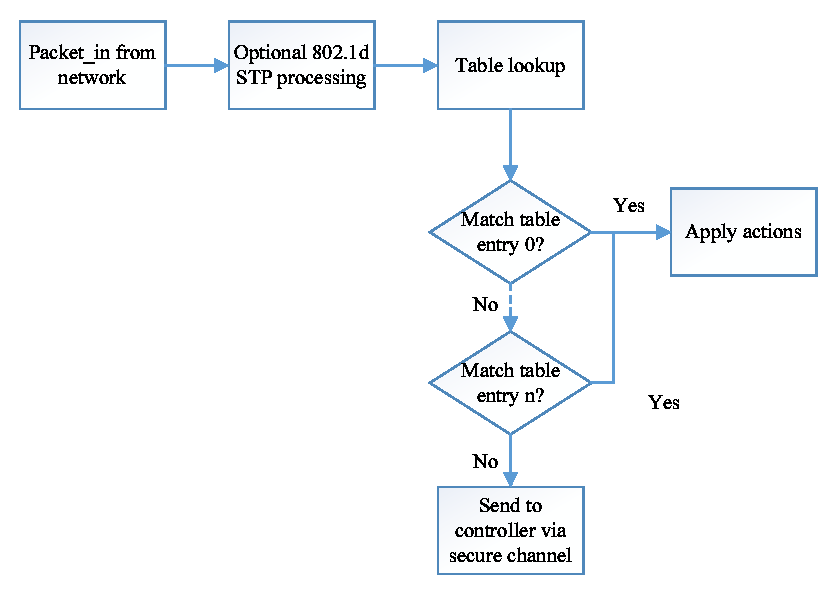
\includegraphics[scale=1]{chap2/switchact.eps}
  \caption{Packet Flow in an OpenFlow Switch}\label{switchact}
\end{figure}

\subsection{The Structure of OpenFlow}
\label{sec:The Structure of OpenFlow}

OpenFlow is the core of SDN ,and basically has the similar structure as SDN. In OpenFlow framework, the most important two parts are the OpenFlow controllers and the OpenFlow switches. Every switch in the network has to connect to at least one controller, and communicates with the controller using standard API. Then the controller runs an application that control and manage the network. Everytime a decision is needed, the OpenFlow switch has to request the OpenFlow controller. For example, if a new packet is send to a switch, the switch will ask the controller how to manage this packet\_in event. Then the controller has to make decisions according to its inside strategies, and tell the switch to forward the packet or just discard it. The structure of OpenFlow can be seen in Figure \ref{opstructure}.

The OpenFlow switch consists of a secure channel and a flow table. After OpenFlow 1.3, the table is changed to a multi-level flow table that has 256 levels. The secure channel is a module that is used for switches to communicate with the controller, and the connnection between switch and controller is realized by sockets. And the flow table is used to save the routing rule of data packets. When data packets come into a switch, it will find the matching rule in the flow table and take corresponding actions. Otherwise, a packet\_in message is generated.

\begin{figure}[htbp]
  \centering
  % Requires \usepackage{graphicx}
  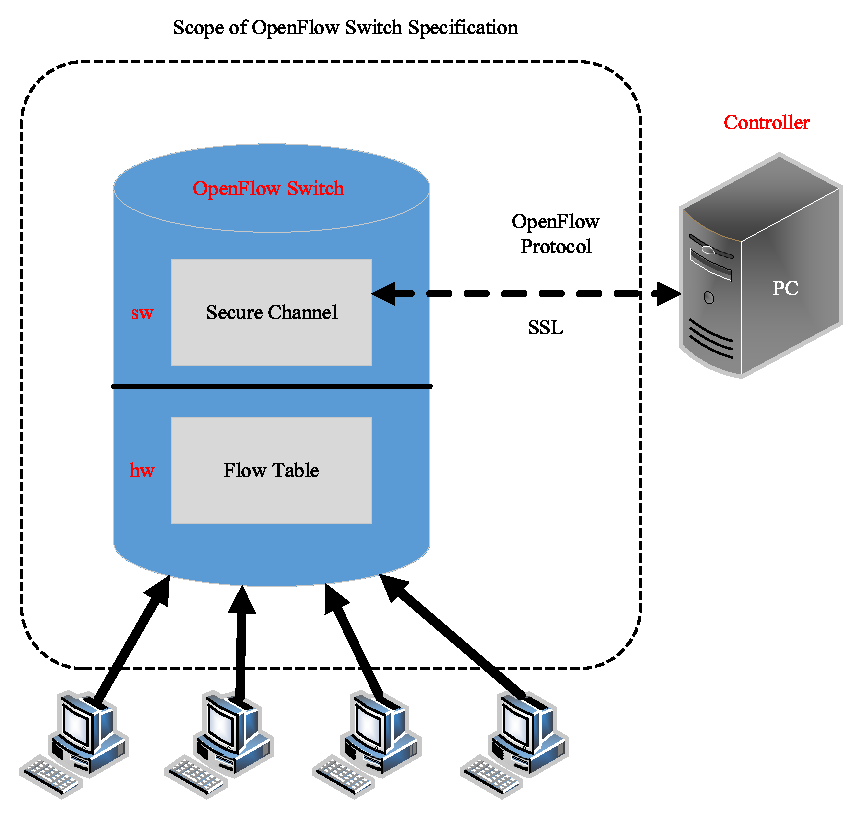
\includegraphics[scale=0.75]{chap2/opstructure.eps}
  \caption{The basic structure of OpenFlow}\label{opstructure}
\end{figure}

Compared to traditional switches, the switches of OpenFlow have a matching level of four, but the traditional switches only have a layer of two. Meanwhile, we can run OpenFlow protocols on OpenFlow switches, and thus implement many functions of a router. Currently, OpenFlow switches can be obtained in three ways: physical OpenFlow switches, installing Open VSwitch (OVS) on physical computers, or using the mininet simulation environments. In this paper, we will use mininet to set up an OpenFlow network and test our algorithms.

There are also many types of OpenFlow controllers, such as pox, ryu, OpenDayLight, etc., which we will compare and discuss later. The controller is mainly divided into three parts in the function level: the communication module in the bottom layer, upper layer applications and the OpenFlow protocols. Since the controller and the switches are linked by sockets, the bottom layer of communication module is also implemented as a socket. And the upper layer applications can be customly developed by users, such as an l2 learning switch.

Another important concept in OpenFlow structure is its port. The port of OpenFlow is a kind of interface with which OpenFlow passes data packets between its controlling process and the rest part of the network. Logically, each pair of switch are connected using an OpenFlow port. The set of OpenFlow port may not be exactly the same as the network port provided by the hardware switch, since some Internet port of the hardware may be disabled by OpenFlow, and OpenFlow may also define extra ports that developers want to use. 

An OpenFlow switch must support three kinds of OpenFlow ports: the physical port, the logical port and the reserved port. The physical ports of OpenFlow are ports defined by switches, corresponding to the hardware ports of a switch. In some kinds of deployments, OpenFlow switches can achieve hardware virtualization of switches. In these conditions, the physical switches of OpenFlow can represent a virtual slice that corresponds to the hardware port of a switch. The logical port of OpenFlow is also defined by switches, but there is not a direct mapping between the logical port and a certain hardware port. It is a higher abstract concept, and may be the ports that do not use OpenFlow in the switches. Meanwhile, the logical ports can be mapped to different physical ports, and the processing of logical ports must be transparent to OpenFlow. The only difference between physical ports and logical ports is that: a data packet sending to a logical port may contain an extra metadata field -- the tunnel ID. And when a message received on the logical port is being sent to the controller, both its logical ports and the physical ports will be acquired by the controller. The reserved port of OpenFlow is used for certain forwarding actions, such as sending to controllers, flooding, or forwarding using methods except OpenFlow, as the traditional switches do.

From the overall point of view, the idea of OpenFlow is in fact quite clear. The network devices maintains a flow table and forward packets according to this flow table. Meanwhile, the generation, maintainment and distribution of this flow table are all implemented by an outside controller. This structure that separates the control plane and data plane means that, for L2 switches, the learning of MAC address will be realized by controller, and the basic L3 routing configurations will also be distributed to switches by this controller. For L3 devices, the Interior gateway protocols (IGP) and the Exterior gateway protocols (EGP) both run on the controller, and are distributed to corresponding routes according to different requirements. The distribution of flow tables can be active as well as passive. In the active pattern, the controller will send the collected information of flow table to network devices once in a while, and later the devices can forward data packets according to the flow table. In the passive pattern, when the network devices receive a message that does not have a match in the flow table, it will send the message to the controller, and let the controller to decide how to forward this message. Then the controller will also distributed related flow tables to the switches.

\section{Principles of Load Balance}
\label{sec:Principles of Load Balance}

Load Balance is a technology that allocates the load to two or more computers, CPU, or other kind of resources adequately in parallel computing, so that we can optimize the resource allocation, maximize the throughput of the processors, and minimize the respond time.

\subsection{Classification of Load Balance}
\label{sec:Classification of Load Balance}

Load Balance is usually classified to several types according to different use cases. In the situation of local traffic management, we usually assort it into two types: static and dynamic. And in the mode of cluster service, we usually divide it to persistent load balance and non-persistent load balance. 

The performance of a cluster is usually directly decided by the design of the balancing schemes. In general, the main duty of the load balance algorithm is to decide how to choose a node in the cluster, and send new coming requests to it, or migrate the jobs to it from other overloaded nodes. There is no omnipotent schems that suits all situations. Thus when we have to design a load balancing strategy, we have to take the features of the cluster, and combine different technologies and algorithms. The basic algorithms used in load balance are listed below:

\textbf{Round Robin} : The Round Robin method is the easiest one to implement in all scheduling algorithms. In a task queue, all the members have the same importance, and the algorithm will choose the next node in sequence. The actions of this algorithm can be predicted, and each node has a possibility of 1/N to be chosen. Thus it is easy to calculate the load distribution in this condition. The Round Robin method is usually used in situations where all the nodes have similar abilities.

\textbf{HASH} : By using an injective and irreversible HASH function, the HASH method send the Internet request to the certain node calculated by the function. The HASH method shows its ability when other load balance algorithms are not very useful, for example, in UDP sessions. 

\textbf{Least Connection Method} : In the Least Connection method, the load balancer records all active connnections, and send the new request to the node that has the least connection at the current time. This method is usually used for problems corresponding to TCP links.

\textbf{Minimum Connection Method} : In Minimum Connection method, the load balancer records the requesting conditions of all nodes during a period of time, and send the next request to the node that has the least total connections during this time. It keeps the number of total connections instead of the current connections, compared to Least Connection Method.

\textbf{Fastest Responding Method} : The load balancer keeps the responding time from itself to each nodes in the cluster, and sends the request to the nodes with the fastest responding speed. In most of the clusters that based on LAN, this method does not perform very well, since the ICMP package can basically respond in 10ms. This means that the difference among different nodes can not be shown very clearly. However, if this method is used on WAN, then it will perform quite well, especially in the topologies that are divergent.

\textbf{Weight Method} : This method can only be used together with other methods. By allocating different values (priorities) to different nodes, it establishes a priority queue. In this queue, nodes with the same priority can be dealed with the Round Robin method or Least Connection method. Here, the priority should be an estimated value based on the ability of each node.

\subsection{Challenges of Load Balance}
\label{sec:Challenges of Load Balance}

Currently portal websites and search engines are becoming more and more popular among people, thus leading to a huge amount of page view every second. This will cause great pressure on the devices of data center networks. Thus, needless to say, devices of load balance are attracting attention from various areas. Nowadays, the load balancers are usually divided into two types: hardware devices, and software load balancers such as Linux Virtual Servers. And most of the network are using both of them. However, we can still discover there are a lot of challenges in this area:

\begin{enumerate}
\item \textbf{The pre-defined trend of load balancer}\\
Since the performance of load balancer may vary a lot in different situations, current load balancers are usually pre-defined for certain applications or certain products. Thus, this condition makes it hard for users to reuse the codes. And users will also meet a lot of trouble if they want to compare different load balancing strategies on these load balancers. Since they are pre-defined, they usually have a strong dependency on a certain kind of structures, preventing users from transplanting it to other platforms.
\item \textbf{The collaboration among multiple load balancers}\\
As the scale of the network increases, a single load balancer cannot satisfy the frequent requests sent by hosts. Thus, the administrator of the network may want to use multiple load balancers to monitor the network. In this way, the processing logic inside each load balancer shall be designed very carefully, considering the potential problem of information sharing, synchronization and control migration.
\item \textbf{The complex hardware and software system}\\
Though we can develop our own software defined load balancers, it will still run on hardwares. Thus, the deployers have to consider the cost of maintaining network devices, or replacing old devices with newer ones. Meanwhile, if the structure of the SDN is changed, there will also be a cost on this update. Of course, the periodical test and update of the algorithm of this load balancer should also be considered.
\end{enumerate}

Refering to the structure of SDN and OpenFlow, we may find that similar problems will occur if we deploy load balance algorithms in it. Thus, there are still a lot to do in this area.

\section{OpenFlow Protocols}
\label{sec:OpenFlow Protocols}

The communication between a switch and a controller is realized using OpenFlow Protocols specified by Open Networking Foundation (ONF) \cite{onf}, by sending a predifined message between them through the secure channel. The secure channel is an port that connects each switch to its controller. When the switch starts, it will start a Transport Layer Security (TLS) connection with the controller defined by users. The switches and controllers will check the status of each other using a certificate. The OpenFlow protocols can be regarded as a possible implemention of switch-controller interactions (the southern interface), since it defines the communication between switch hardware and network controllers. However, some fine grained security choices are still not concerned in current standards.

OpenFlow protocols defined three kinds of message types, each can be further devided into several subtypes: controller-to-switch, symmetric, asynchronous. 

\subsection{Controller-to-switch Messages}
\label{sec:Controller-to-switch Messages}

The controller-to-switch message is started by the switch, and is used for directly managing the switches or check the status of switches. This kind of message may or may not require a response and can be divided to the following subtypes:

\textbf{Features} : When establshing a TLS session, the controller will send a feature request to the switch, and the switch must answer the request using a feature message. The message will include the functions that the switch supports in detail.

\textbf{Configuration} : Controllers can set and query the configuration parameters in the switch, and the switch will only respond to the query message.

\textbf{Modify-State}: This message is sent by controller, and is used for managing the state of switches. We can use this message to add, modify or delete the flow entries in the flow table, or set the priority of switch ports. 

\textbf{Read-State} : This kind of message collects statistics from the flow table, ports or flow entries from the switch.

\textbf{Packet-Out} : Controllers use this message to send packets from a designated port of switch.

\textbf{Barrier}: Controllers use a Barrier request and the response to make sure the dependency of information, or receive the notification that the actions are completed. We will use this message for synchronization purpose in our scheme.

\subsection{Symmetric Messages}
\label{sec:Symmetric Messages}

Symmetric messages can be sent from a controller to a switch, and can also be sent from a switch to a controller. There are usually three types of symmetric messages:

\textbf{Hello} : The Hello message is used for controllers and switches to establish a connection. After the connection is set up, they will send each other a Hello message to make sure the success.

\textbf{Echo} : Both controllers and switches can send an Echo message to the other side. The receiver must reply the message. This message is used for testing delays and check whether the connection is still kept. In other words, it can be used for 'heartbeat' messages.

\textbf{Vender} : The Vender message is always kept for future versions. It makes use of the OpenFlow space and intends to offer a standard way to extend the function of OpenFlow.

\subsection{Asynchronous Messages}
\label{sec:Asynchronous Messages}

The asynchronous messages are started by the switches, and is used for notifying controllers the network events and the changes of switches' status. A switch sends the asynchronous message to the controller when a data packet arrives, the status of the switch changes, or an error occurs. Four types of Asynchronous messages are usually seen:

\textbf{Packet-in} : When switches receives a packet, it will try to find a match in its flow table, and then follow the actions defined in that flow entry. However, if no matches are found, or if the packet is required to be sent to the controller, the switch will then send a packet-in message to the controller. For switches that have enough space to store this packet, it will include the part of the header field and the buffer ID in the packet-in message. Otherwise, the switch must include all the data of that packet in this packet-in message.

\textbf{Flow-removed} : As we have said before, there is a limited space for flow tables to store the flow entries. Thus when the flow table is full and a new entry is to be added, the counters will find the most inactive flow entry and delete that. And in fact, each flow entry have a life period, the switch will delete that entry if it exceeds its living time. In these two conditions, the switch will generate a flow-removed message.

\textbf{Port-status} : When the configuration status of a switch changes, it will send a port-status message to the controller.

\textbf{Error} : This message is used to notify the controller that there is an error.

\subsection{Communication Process}
\label{sec:Communication Process}

When an OpenFlow connection is established, both the controllers and the switches have to send an OFPT\_HELLO message to the other side. This message will include the highest version number of supported OpenFlow protocols in each side. The receiver will use the lowest protocol version that is supported by both side. As soon as a sharing version number is found, the connection will be established successfully. Else an OFPT\_ERROR message will be sent and breaks the link.

When an error occurs, the switch will attempt to connect to the backup controller. If all the attemptions fail in the end, the switch will come into the emergency model, and reset all the TCP links. Only flow entries of the emergency model will be matched during this time, and all other entries will be deleted.

\subsection{Role of controllers in a multiple controller situation}
\label{sec:Role of controllers in a multiple controller situation}

Multiple controllers are supported in OpenFlow 1.3 \cite{opproto}. However, this multiple controller situation is only meaningful for the switches. Since OpenFlow is a protocol used for communication between controllers and switches. The communication between controllers and how the controllers cooperate is not concerned in OpenFlow.

Compared with the switches, the controllers have three types of roles in OpenFlow 1.3: equal, master and slave. A controller can change its role at any time.

\textbf{OFPCR\_ROLE\_EQUAL} : This means the controller is an equal controller. It has all of the permissions, and has the same role as other equal controlles. For example, if a switch connects to three controllers, and the role of all these controllers are equal. Then any one of the controllers has the same importance for the switch.
\textbf{OFPCR\_ROLE\_SLAVE} : This means the controller has the role as a slave. It has read-only permissions, and does not receive asychronous messages except for port\_status message. Meanwhile, this controller cannot send following messages (messages for writing purpose): packet\_out, flow\_mod, group\_mod, port\_mod, table\_mod\_request and table\_features. An error message must be replied if a switch receives above messages from a slave controller. There can be many slave controllers in the network.

\textbf{OFPCR\_ROLE\_MASTER} : This means the controller is a master controller. It has the same permission as an equal controller. The only difference is that, there can only be one master controller in the system, but can have many equal controllers.

\subsection{Evolvement of OpenFlow Versions}
\label{sec:Evolvement of OpenFlow Versions}

Since OpenFlow 1.0 has been released in 2009, this protocol has experienced an obvious evolvement in its following versions 1.1, 1.2, 1.3 and 1.4. The currently most popular version is OpenFlow 1.0, and OpenFlow 1.3 is also accepted by more and more companies. Figure \ref{evolvement} shows the difference between these two versions.

\begin{figure}[htbp]
  \centering
  % Requires \usepackage{graphicx}
  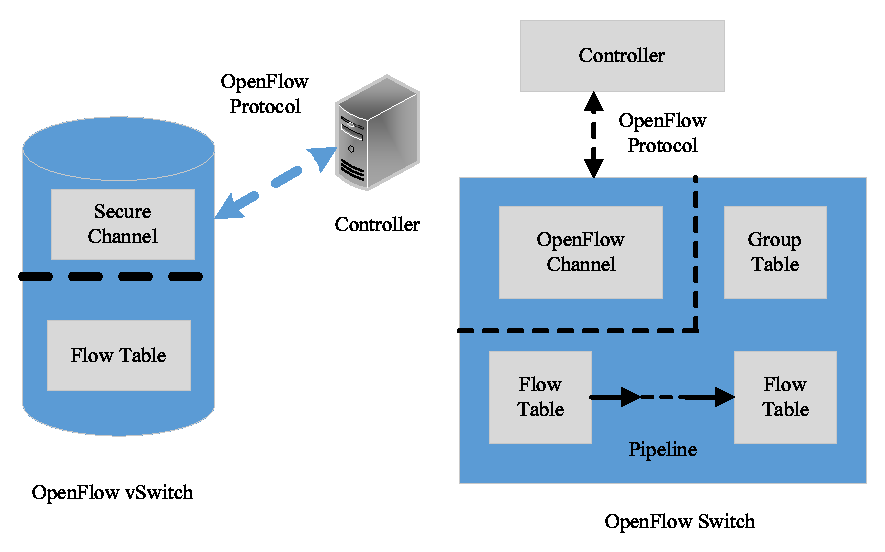
\includegraphics[scale=1]{chap2/evolvement.eps}
  \caption{The difference between OpenFlow version 1.0 and 1.3}\label{evolvement}
\end{figure}

Let us have a short review of the evolvement history of OpenFlow, which is quite important if we want to make a research on multiple controllers in OpenFlow network.

In OpenFlow 1.0, there is a flow table in every OpenFlow switch, which is used for searching, processing and forwarding the packets. Each switch is only allowed to communicate with one controller, and the maintainment of the flow table is also realized by corresponding OpenFlow messages sent by the controller. The advantage of this version is that it is totally compatible with current commmercial chips. Companies can deploy OpenFlow 1.0 in their traditional switches, just by updating the firmware. Thus, OpenFlow 1.0 is the most popular version nowadays.

From the version of OpenFlow 1.1, this protocol begins to support multi-level flow tables. By dividing the flow table matching process into several steps and make it working in a streamline, we can avoid the problem that a single flow table is over-expanded with so much information. Meanwhile, the concept of Group is also used in OpenFlow 1.1, making it possible to perform the same actions by citing the same group tables in different flow entries.

Then in OpenFlow 1.2, users are allowed to define their own matching fields, under the definition of OpenFlow Extensible Match (OXM). Meanwhile, in this version, a switch is allowed to connect with several controllers, and the controllers are allowed to change their role by sending ROLE\_REQUEST messages.

In April, 2012, another long-term support version OpenFlow 1.3 is released. In this version, more matching keywords are allowed. And it permits controllers and switches to decide the protocol versions to be used, by negotiating in the start phase of the connection. One year later, OpenFlow 1.4 was released, and made several improvements in the control plane, but was still based on OpenFlow 1.3.

\section{Controllers used in OpenFlow network}
\label{sec:Controllers used in OpenFlow network}

Several kinds of controllers are widely used at the moment. Among them, POX, OpenDayLight, Floodlight, Beacon and Ryu are the most popular ones. In this experiment, we will use Ryu controller to monitor the whole network. Other controllers will be introduced and compared later.

\subsection{Introduction to Ryu}
\label{sec:Introduction to Ryu}

Ryu \cite{ryu} is a SDN controller developed by Nippon Telegraph \& Telephone (NTT) in Japan.
This controller is implemented by Python, and users can realize their own applications using Python. Ryu has support for several versions of OpenFlow at the moment, including OpenFlow 1.0, OpenFlow 1.2 and OpenFlow 1.3, It also has support for deploying applications on OpenStack. The application programming model of Ryu is shown in Figure \ref{ryueps}.

\begin{figure}[htbp]
  \centering
  % Requires \usepackage{graphicx}
  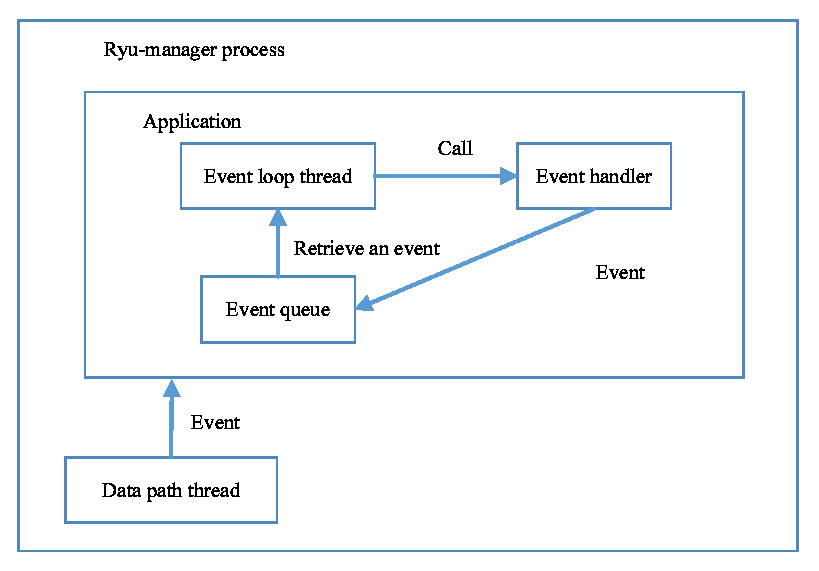
\includegraphics[scale=1]{chap2/ryu.eps}
  \caption{Application programming model of Ryu}\label{ryueps}
\end{figure}

The code of the main controller is organized under the /ryu/ryu/ folder. Let's have a short introduce on the main structure of Ryu code.

\begin{itemize}
\item app/ - Contains several applications that can run directly on the controller
\item base/ - Contains the basic classes of applications. The most important document in this folder is app\_manager.py. This document is the central manager of an Ryu application, which is used for loading the application, receiving messages and finishing the routing. The RyuApp class is defind in this file.
\item controller/ - Contains several important files to handle OpenFlow functions, such as events.py, ofp\_handler.py, controller.py, etc. The basic class OpenFlowController is defined in controller.py, which is used to define an OpenFlow controller and dealing with connections between controllers and switches.
\item lib/ - Defines the basic data structures, such as dpid, mac and ip.
\item ofproto/ - Contains two types of files: the definition of the data structure of OpenFlow protocols, and the related parsers for these protocols. 
\item topology/ - Contains codes for discovering the topology of OpenFlow network.
\end{itemize}

Then we used the hub application as an example to elucidate how to write a controller application in Ryu. The code is as follows:

\begin{lstlisting}[language={python}, caption={hub.py written by Ryu}]
from ryu.base import app_manager
from ryu.controller import ofp_event
from ryu.controller.handler import MAIN_DISPATCHER
from ryu.controller.handler import set_ev_cls

class L2Switch(app_manager.RyuApp):
    def __init__(self, *args, **kwargs):
        super(L2Switch, self).__init__(*args, **kwargs)

    @set_ev_cls(ofp_event.EventOFPPacketIn, MAIN_DISPATCHER)
    def packet_in_handler(self, ev):
        msg = ev.msg
        datapath = msg.datapath
        ofp = datapath.ofproto
        ofp_parser = datapath.ofproto_parser

        actions = [ofp_parser.OFPActionOutput(ofp.OFPP_FLOOD)]
        out = ofp_parser.OFPPacketOut(
            datapath=datapath, buffer_id=msg.buffer_id, in_port=msg.in_port,
            actions=actions)
        datapath.send_msg(out)
\end{lstlisting}

In this code, we import ofp\_event at first. ofp\_event is used to define an event, so that we can register a handler in the function and monitor the events as well as reply to them. The main function in this file -- packet\_in\_handler is used to deal with packet\_in events. And we use the signal @set\_ev\_cls to tell Ryu that, when the controller receives a packet\_in event, it will resort to packet\_in\_handler. MAIN\_DISPATCHER represents a general status. The first parameter of set\_ev\_cls represents the function to be used when event happens, and the second parameter tells the switch that, the function can only be called after the connection succeeds.

Then in the function of packet\_in\_handler, ev represents for an event, and ev.msg is a member of ev, which is used to carry the packet that triggers the event. The msg parameter is in fact a packet\_in message, and msg.datapath is used to get the datapath structure of msg, which is used to describe a network bridge. datapath.ofproto is an object of OpenFlow protocol structure, and contains the data structure used later. datapath.ofp\_parser is a data structure used to parse that object. And actions is a list, which stores the actions to be done in the future. The parameter out in this code is a packet\_out structure, containing the necessary informations of how to deal with the packet, and the function datapath.send\_msg() will send the data to the designated datapath.

\subsection{Other popular controllers}
\label{sec:Other popular controllers}

\textbf{POX} : The first OpenFlow controller is NOX written by C++,and POX is a Python-version NOX that only supports developing using Python. We can thus regard POX as a general, open-source OpenFlow controller written by Python. It is also a platform on which users can develop Internet applications and establish their own topologies. The main application area for POX is the researching area. Since most of the researches will not last for a long time, thus POX devotes to provide users with adequate interfaces instead of stable interfaces.

\textbf{Beacon} : Beacon is a fast, cross-platform and modularized controller based on Java. This controller not only supports event-driven actions, but also supports actions that are based on threads. The controller, whose developing process began in 2010, is not used in some researching projects and platforms for experiments. Since Beacon is written by Java, it is capable of running on several platforms such as Linux and Android. Another advantage of Beacon is that, we can start, stop, install or refresh the modules of Beacon even if it is running, and these actions will not influence other unrelated modules.

\textbf{Floodlight} : Floodlight Open SDN Controller is another kind of OpenFlow controller that is written by Java, usually used in enterprise-level applications. Floodlight runs in Java Virtual Machines (JVM), so it may be a little slower than other controller written in C++ or Python. Floodlight is not only a controller, but also a set of applications running on Floodlight controller. Thus Floodlight is usually considered to be composed of three parts: the Floodlight controller, the application compiled with the controller as a Java module, and the network applications over the REST API of Floodlight.

\textbf{OpenDayLight} : OpenDayLight (ODL) controller is a modularized, multi-protocol controller infrastructure that has a high scalability in both scales and functions. It is developed by Java, and can run on any hardware platform that supports Java JVM 1.7 or higher, in the form of a Java virtual machine. OpenDayLight controller not only supports OpenFlow protocols, but also supports other open-source protocols. Meanwhile, it allows communication with other devices with OpenFlow or other protocol agents. Its northern API also supports the collaboration of user defined applications and the controller itself in controlling the network.
